
\documentclass[letterpaper,hide notes,xcolor={table,svgnames},pdftex,10pt]{beamer}
\def\showexamples{t}

\usecolortheme{crane}
\setbeamertemplate{navigation symbols}{}

\usetheme{MyPittsburgh}
\usepackage{hyperref}
\usepackage{graphicx,xspace}
\usepackage[normalem]{ulem}
\usepackage{multicol}
\usepackage{amsmath,amssymb,amsthm,graphicx,xspace}
\newcommand\SF[1]{$\bigstar$\footnote{SF: #1}}

\usepackage[sfdefault,lf]{carlito}
\usepackage[T1]{fontenc}
\usepackage[scaled]{beramono}
\usepackage{tikzpagenodes}
\newcommand{\Rplus}{\protect\hspace{-.1em}\protect\raisebox{.35ex}{\small{\small\textbf{+}}}}
\newcommand{\Cpp}{\mbox{C\Rplus\Rplus}\xspace}

\newcounter{tmpnumSlide}
\newcounter{tmpnumNote}

\newcommand\mnote[1]{%
	\addtocounter{tmpnumSlide}{1}
	\ifdefined\showcues {~\tiny\fbox{\arabic{tmpnumSlide}}}\fi
	\note{\setlength{\parskip}{1ex}\addtocounter{tmpnumNote}{1}\textbf{\Large \arabic{tmpnumNote}:} {#1\par}}}

\newcommand\mmnote[1]{\note{\setlength{\parskip}{1ex}#1\par}}


\newcommand\mquestion[2]{{~\color{red}\fbox{?}}\note{\setlength{\parskip}{1ex}\par{\Large \textbf{?}} #1} \note{\setlength{\parskip}{1ex}\par{\Large \textbf{A}} #2\par}\ifdefined \presentationonly \pause \fi}

\newcommand\blackboard[1]{%
	\ifdefined   \showblackboard
		{#1}
	\else {\begin{center} \fbox{\colorbox{blue!30}{%
						\begin{minipage}{.95\linewidth}%
							\hspace{\stretch{1}} Some space intentionally left blank; done at the blackboard.%
						\end{minipage}}}\end{center}}%
	\fi%
}

\usepackage{listings}
\lstset{%
	keywordstyle=\bfseries,
	aboveskip=15pt,
	belowskip=15pt,
	captionpos=b,
	identifierstyle=\ttfamily,
	frame=lines,
	numbers=left, basicstyle=\scriptsize, numberstyle=\tiny, stepnumber=0, numbersep=2pt}

\usepackage{siunitx}
\newcommand\sius[1]{\num[group-separator = {,}]{#1}\si{\micro\second}}
\newcommand\sims[1]{\num[group-separator = {,}]{#1}\si{\milli\second}}
\newcommand\sins[1]{\num[group-separator = {,}]{#1}\si{\nano\second}}
\sisetup{group-separator = {,}, group-digits = true}

%% -------------------- tikz --------------------
\usepackage{tikz}
\usetikzlibrary{positioning}
\usetikzlibrary{arrows,backgrounds,automata,decorations.shapes,decorations.pathmorphing,decorations.markings,decorations.text}

\tikzstyle{place}=[circle,draw=blue!50,fill=blue!20,thick, inner sep=0pt,minimum size=6mm]
\tikzstyle{transition}=[rectangle,draw=black!50,fill=black!20,thick, inner sep=0pt,minimum size=4mm]

\tikzstyle{block}=[rectangle,draw=black, thick, inner sep=5pt]
\tikzstyle{bullet}=[circle,draw=black, fill=black, thin, inner sep=2pt]

\tikzstyle{pre}=[<-,shorten <=1pt,>=stealth',semithick]
\tikzstyle{post}=[->,shorten >=1pt,>=stealth',semithick]
\tikzstyle{bi}=[<->,shorten >=1pt,shorten <=1pt, >=stealth',semithick]

\tikzstyle{mut}=[-,>=stealth',semithick]

\tikzstyle{treereset}=[dashed,->, shorten >=1pt,>=stealth',thin]

\usepackage{ifmtarg}
\usepackage{xifthen}
\makeatletter
% new counter to now which frame it is within the sequence
\newcounter{multiframecounter}
% initialize buffer for previously used frame title
\gdef\lastframetitle{\textit{undefined}}
% new environment for a multi-frame
\newenvironment{multiframe}[1][]{%
	\ifthenelse{\isempty{#1}}{%
		% if no frame title was set via optional parameter,
		% only increase sequence counter by 1
		\addtocounter{multiframecounter}{1}%
	}{%
		% new frame title has been provided, thus
		% reset sequence counter to 1 and buffer frame title for later use
		\setcounter{multiframecounter}{1}%
		\gdef\lastframetitle{#1}%
	}%
	% start conventional frame environment and
	% automatically set frame title followed by sequence counter
	\begin{frame}%
		\frametitle{\lastframetitle~{\normalfont(\arabic{multiframecounter})}}%
		}{%
	\end{frame}%
}
\makeatother

\makeatletter
\newdimen\tu@tmpa%
\newdimen\ydiffl%
\newdimen\xdiffl%
\newcommand\ydiff[2]{%
	\coordinate (tmpnamea) at (#1);%
	\coordinate (tmpnameb) at (#2);%
	\pgfextracty{\tu@tmpa}{\pgfpointanchor{tmpnamea}{center}}%
	\pgfextracty{\ydiffl}{\pgfpointanchor{tmpnameb}{center}}%
	\advance\ydiffl by -\tu@tmpa%
}
\newcommand\xdiff[2]{%
	\coordinate (tmpnamea) at (#1);%
	\coordinate (tmpnameb) at (#2);%
	\pgfextractx{\tu@tmpa}{\pgfpointanchor{tmpnamea}{center}}%
	\pgfextractx{\xdiffl}{\pgfpointanchor{tmpnameb}{center}}%
	\advance\xdiffl by -\tu@tmpa%
}
\makeatother
\newcommand{\copyrightbox}[3][r]{%
	\begin{tikzpicture}%
		\node[inner sep=0pt,minimum size=2em](ciimage){#2};
		\usefont{OT1}{phv}{n}{n}\fontsize{4}{4}\selectfont
		\ydiff{ciimage.south}{ciimage.north}
		\xdiff{ciimage.west}{ciimage.east}
		\ifthenelse{\equal{#1}{r}}{%
			\node[inner sep=0pt,right=1ex of ciimage.south east,anchor=north west,rotate=90]%
			{\raggedleft\color{black!50}\parbox{\the\ydiffl}{\raggedright{}#3}};%
		}{%
			\ifthenelse{\equal{#1}{l}}{%
				\node[inner sep=0pt,right=1ex of ciimage.south west,anchor=south west,rotate=90]%
				{\raggedleft\color{black!50}\parbox{\the\ydiffl}{\raggedright{}#3}};%
			}{%
				\node[inner sep=0pt,below=1ex of ciimage.south west,anchor=north west]%
				{\raggedleft\color{black!50}\parbox{\the\xdiffl}{\raggedright{}#3}};%
			}
		}
	\end{tikzpicture}
}


%% --------------------

%\usepackage[excludeor]{everyhook}
%\PushPreHook{par}{\setbox0=\lastbox\llap{MUH}}\box0}

%\vspace*{\stretch{1}

%\setbox0=\lastbox \llap{\textbullet\enskip}\box0}

\setlength{\parskip}{\fill}

\newcommand\noskips{\setlength{\parskip}{1ex}}
\newcommand\doskips{\setlength{\parskip}{\fill}}

\newcommand\xx{\par\vspace*{\stretch{1}}\par}
\newcommand\xxs{\par\vspace*{2ex}\par}
\newcommand\tuple[1]{\langle #1 \rangle}
\newcommand\code[1]{{\sf \footnotesize #1}}
\newcommand\ex[1]{\uline{Example:} \ifdefined \presentationonly \pause \fi
	\ifdefined\showexamples#1\xspace\else{\uline{\hspace*{2cm}}}\fi}

\newcommand\ceil[1]{\lceil #1 \rceil}


\AtBeginSection[]
{
	\begin{frame}
		\frametitle{Outline}
		\tableofcontents[currentsection]
	\end{frame}
}



\pgfdeclarelayer{edgelayer}
\pgfdeclarelayer{nodelayer}
\pgfsetlayers{edgelayer,nodelayer,main}

\tikzstyle{none}=[inner sep=0pt]
\tikzstyle{rn}=[circle,fill=Red,draw=Black,line width=0.8 pt]
\tikzstyle{gn}=[circle,fill=Lime,draw=Black,line width=0.8 pt]
\tikzstyle{yn}=[circle,fill=Yellow,draw=Black,line width=0.8 pt]
\tikzstyle{empty}=[circle,fill=White,draw=Black]
\tikzstyle{bw} = [rectangle, draw, fill=blue!20,
text width=4em, text centered, rounded corners, minimum height=2em]

\newcommand{\CcNote}[1]{% longname
	This work is licensed under the \textit{Creative Commons #1 3.0 License}.%
}
\newcommand{\CcImageBy}[1]{%
	\includegraphics[scale=#1]{creative_commons/cc_by_30.pdf}%
}
\newcommand{\CcImageSa}[1]{%
	\includegraphics[scale=#1]{creative_commons/cc_sa_30.pdf}%
}
\newcommand{\CcImageNc}[1]{%
	\includegraphics[scale=#1]{creative_commons/cc_nc_30.pdf}%
}
\newcommand{\CcGroupBySa}[2]{% zoom, gap
	\CcImageBy{#1}\hspace*{#2}\CcImageNc{#1}\hspace*{#2}\CcImageSa{#1}%
}
\newcommand{\CcLongnameByNcSa}{Attribution-NonCommercial-ShareAlike}

\newenvironment{changemargin}[1]{% 
	\begin{list}{}{% 
		\setlength{\topsep}{0pt}% 
		\setlength{\leftmargin}{#1}% 
		\setlength{\rightmargin}{1em}
		\setlength{\listparindent}{\parindent}% 
		\setlength{\itemindent}{\parindent}% 
		      \setlength{\parsep}{\parskip}% 
		      }% 
		\item[]}{\end{list}}




\title{Lecture 6 --- Inter-Process Communication}

\author{Jeff Zarnett \\ \small \texttt{jzarnett@uwaterloo.ca}}
\institute{Department of Electrical and Computer Engineering \\
	University of Waterloo}
\date{\today}


\begin{document}

\begin{frame}
	\titlepage

\end{frame}

\begin{frame}
	\frametitle{IPC Motivation}

	When 2+ processes would like to co-ordinate/exchange data the mechanism is called \alert{inter-process communication}.

	If a process shares data with another process in the system, the operating system will provide some facilities to make this possible.

	The motivations for inter-process communication are fairly obvious.

	\begin{center}
		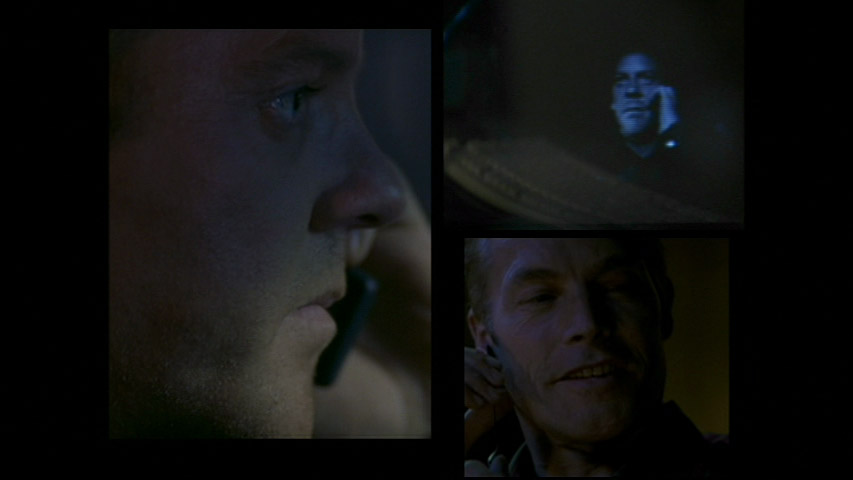
\includegraphics[width=0.6\textwidth]{images/24-splitscreen.jpg}
	\end{center}

\end{frame}


\begin{frame}
	\frametitle{IPC Preliminaries}

	Before proceeding, we need to define some things.

	It is the transfer of data from one process to another.

	The data being transferred is typically referred to as the \textit{message}.

	The process sending that message is the \textit{sender}.

	The process receiving it will be the \textit{receiver}.

	This terminology may seem (painfully) obvious.

\end{frame}


\begin{frame}
	\frametitle{Thanks!}

	\begin{center}
		
\includegraphics[width=0.8\textwidth]{images/thanks-captain-obvious}
	\end{center}


\end{frame}


\begin{frame}
	\frametitle{IPC: What to Send}

	The processes involved must have some agreement on:\\
	\quad What data a message should contain; and\\
	\quad The way the data is formatted.

	There may be defined standards, e.g., XML.

	The processes themselves must be aware the message is in XML format.

	How this agreement is made falls outside the purview of the OS.

\end{frame}

\begin{frame}
	\frametitle{Messages: (A)synchronous}

	Sending and receiving of messages may be either synchronous or asynchronous.

	Synchronous Send: the sender sends the message and then is blocked from proceeding until the message is received.

	Asynchronous Send: the sender can post the message and then carry on.

	Synchronous Receive: the receiver is blocked until it receives a message.

	Asynchronous Receive: the receiver is notified there is no message available and continues execution.

\end{frame}

\begin{frame}
	\frametitle{Messages: (A)synchronous}

	Thus there are four combinations to consider, three of which are common:

	\begin{enumerate}
		\item \textbf{Synchronous send, synchronous receive}
		\item \textbf{Synchronous send, asynchronous receive}
		\item \textbf{Asynchronous send, synchronous receive}
		\item \textbf{Asynchronous send, asynchronous receive}
	\end{enumerate}

	We may also have ``acknowledgement'' messages.

\end{frame}

\begin{frame}
	\frametitle{Producer-Consumer Problem}

	A general paradigm for understanding IPC is known as the \textit{producer-consumer} problem.

	The \alert{producer} creates some information.

	The information is later used by the \alert{consumer}.

	Example: the database produces data to be consumed by the shell.

	This is a general problem and applicable to client-server situations.

\end{frame}

\begin{frame}
	\frametitle{IPC Implementation Strategies}

	There are three approaches we will consider on how we can accomplish IPC:
	\begin{enumerate}
		\item Shared memory.
		\item The file system.
		\item Message passing.
	\end{enumerate}

	All are quite common.

\end{frame}


\begin{frame}
	\frametitle{Shared Memory}
	\begin{center}
		
\includegraphics[width=0.7\textwidth]{images/mindmeld.jpg}
	\end{center}

\end{frame}


\begin{frame}
	\frametitle{Shared Memory}

	Conceptually, the idea of shared memory is very simple.

	A region of memory is designated as being shared with some processes.

	Those processes may read and write to that location.

	To share an area of memory, the OS must be notified.

\end{frame}

\begin{frame}
	\frametitle{Shared Memory}
	Normally, a region of memory is associated with exactly one process (its owner).

	That process may read and write that location.\\
	\quad Other processes may not.

	If a second process attempts to do so, the operating system will intervene and that will be an error.

	If a process wants to designate memory as shared, it needs to tell the operating system it is okay.

\end{frame}

\begin{frame}
	\frametitle{Shared Memory}

	The OS needs to know that the memory is referenced by two processes.

	If the first one terminates and is reaped, the memory may still be in use by the second process.

	The previously-shared region should not be considered free as long as the second process is still using it.

	Once the area of memory is shared, when either process attempts to access it, it is just a normal memory access.

	The kernel is only involved in the setup and cleanup of that shared area.

\end{frame}

\begin{frame}
	\frametitle{Shared Memory}

	\begin{center}
		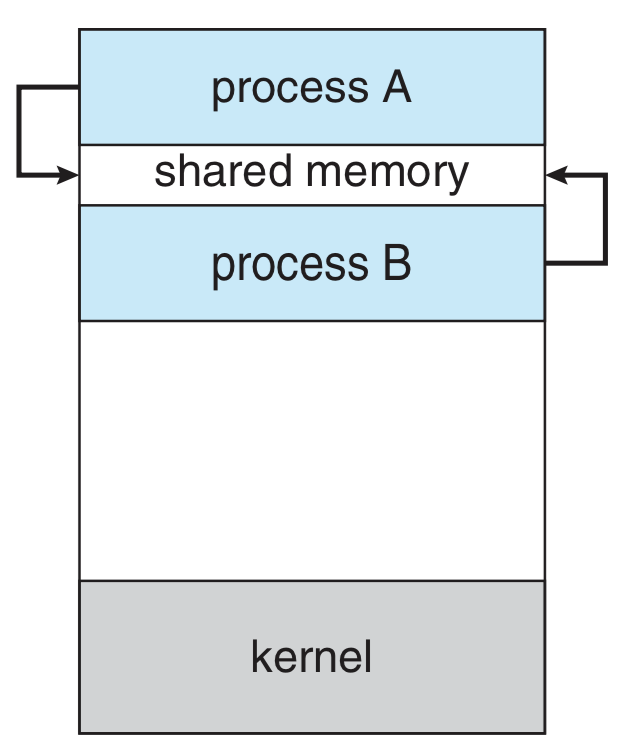
\includegraphics[width=0.6\textwidth]{images/shared-memory.png}
	\end{center}

\end{frame}

\begin{frame}
	\frametitle{Shared Memory: Risk}

	When a section of memory is shared, there is the possibility that one process overwrites another's changes.

	To prevent this, we need a system of co-ordination.

	...A subject we will return to later.

\end{frame}


\begin{frame}
	\frametitle{File System}

	\begin{center}
		
\includegraphics[width=0.7\textwidth]{images/datatape.jpg}
	\end{center}

\end{frame}


\begin{frame}
	\frametitle{File System}

	Another way for 2 processes to communicate is through the file system.

	Unlike shared memory, messages stored in the file system are persistent.

	Can be used if the sender \& receiver know nothing about one another.

\end{frame}

\begin{frame}
	\frametitle{File System}

	The producer may write to a file in an agreed upon location.

	The consumer may read from that same location.

	The operating system is still involved because of its role in file creation and manipulation.

\end{frame}

\begin{frame}
	\frametitle{File System: Co-ordination}

	If one file is being used then we still have the problem of co-ordination.

	We can get around this, however, by using multiple files with unique IDs.

	Example from a co-op work term: if the producer is generating XML data, it can write in a file in a designated \texttt{import/} directory.

	The consumer program scans the directory, and imports files.

	In this case, since one process writes files and another reads them, there is no possibility that one process overwrites the data of another.

	If the sender chooses distinct file names, it will not overwrite a message if a second message is created before the receiver picks up the first.

\end{frame}


\begin{frame}
	\frametitle{Message Passing}

	\begin{center}
		
\includegraphics[width=0.7\textwidth]{images/communicator.jpg}
	\end{center}

\end{frame}


\begin{frame}
	\frametitle{Message Passing}

	Message passing is a service provided by the operating system.

	The sender will give the message to the OS and ask that it be delivered to a recipient.

	There are two basic operations: sending and receiving.

	Messages can be of fixed or variable size.


\end{frame}

\begin{frame}
	\frametitle{Message Passing}

	Our experience with postal mail, or e-mail, suggests that to send a message successfully, the sender needs to indicate where the message should go.

	Under \textit{direct communication}, each process that wants to communicate needs to explicitly name the recipient or sender of the communication.

	We have to know some identifier for the other processes; not very flexible.
\end{frame}

\begin{frame}
	\frametitle{Signals}

	Signals are interrupts with a specified ID.

	\begin{center}
		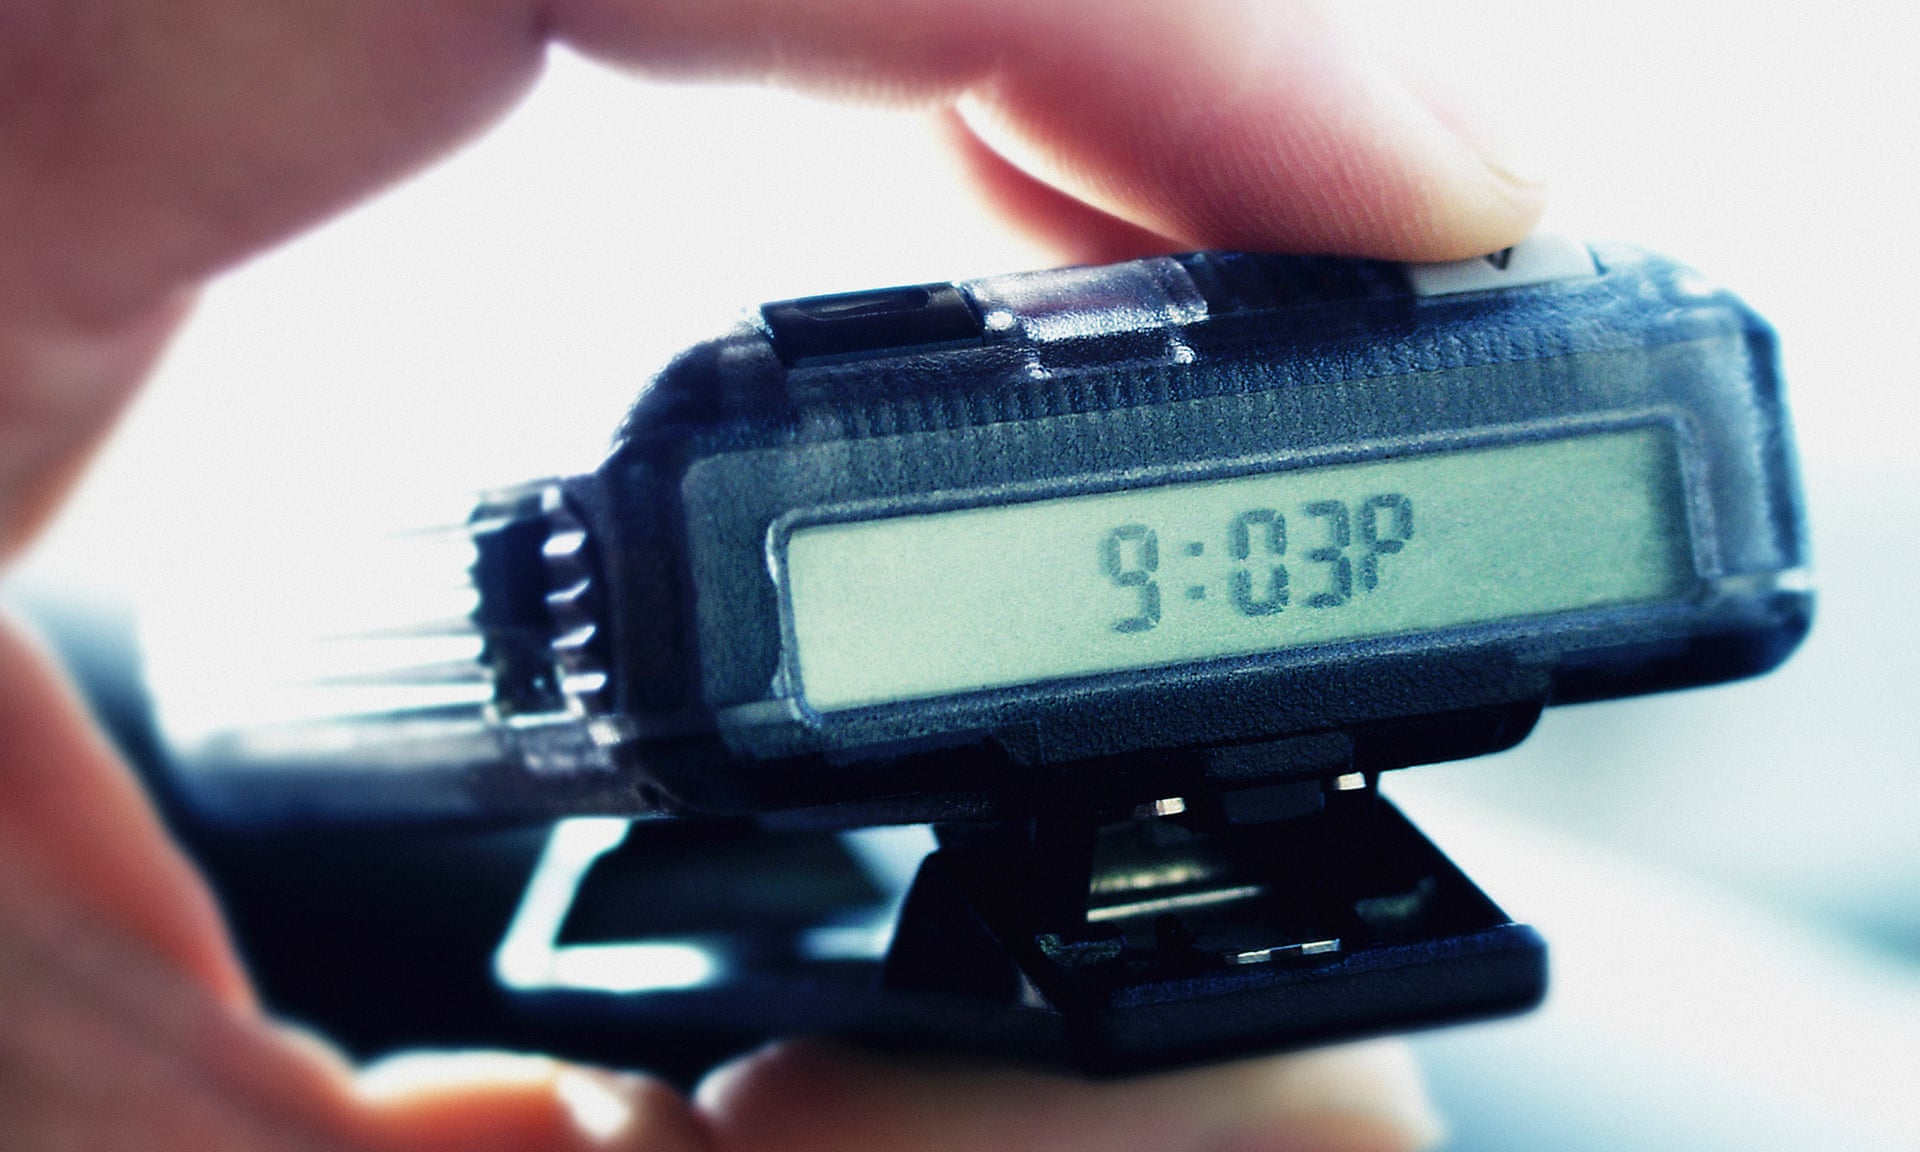
\includegraphics[width=0.6\textwidth]{images/pager.jpg}\\
		Image Credit:  Steven Puetzer/Getty Images
	\end{center}

	They don't really contain a message.

\end{frame}


\begin{frame}
	\frametitle{Signal: No Message}

	The fact that a signal contains no message is a limitation that means signals can't be used for every single interprocess communication scenario.

	When the fire alarm sounds in a building, you don't need an accompanying voice announcement!

	Why?

\end{frame}



\begin{frame}
	\frametitle{Signal: Preparation}

	You have previously been informed that when the fire alarm sounds it means you need to exit the building.

	Signals: you need to know what to listen for and what's supposed to happen if you want to react accordingly.

\end{frame}


\begin{frame}
	\frametitle{Programmatic Signals}

	The appropriate header for including signals is \texttt{signal.h}.

	It contains the definitions that let you write \texttt{SIGKILL} instead of having to put an explicit int \texttt{9}.

	Unfortunately there is not always 100\% agreement between different implementations about what the higher signal numbers mean.

\end{frame}


\begin{frame}[fragile]
	\frametitle{Programmatic Signals}

	There are two functions for sending a signal programmatically:

	\begin{lstlisting}[language=C]
int kill( int pid, int signo );
int raise( int signo );
\end{lstlisting}

	Both functions return 0 if they were successful and -1 if they were unsuccessful.

	The \texttt{raise} function sends the signal to the current process.

\end{frame}


\begin{frame}
	\frametitle{Finding the Identity of a Stranger}

	We need to know the process ID of the recipient.

	But how do processes find one another's IDs? Registration!

	mysql (a database) server will put its process ID in the file \texttt{/var/run/mysqld/mysqld.pid}.

	In that file is just the number of its process ID (e.g., \texttt{1494}).

	Any other communication method will work!

\end{frame}


\begin{frame}
	\frametitle{Why not Function Overload?!}

	The \texttt{kill} function does different things depending on its first argument.

	\begin{itemize}
		\item \texttt{pid > 0}
		\item \texttt{pid == 0}
		\item \texttt{pid == -1}
		\item \texttt{pid < -1}
	\end{itemize}

\end{frame}

\begin{frame}
	\frametitle{The Null Signal}

	You can also invoke the \texttt{kill} function with a 0 argument for the signal.

	This is called the \alert{null signal}.

	It does not actually send any signal, but can be used to check if the recipient process exists.

	But beware: process IDs are only relatively unique!

\end{frame}


\begin{frame}
	\frametitle{Did You Get My Text?!}

	A process can only actually deal with a signal when that process is running.

	A signal is generated by something, and it is later delivered to the recipient.

	But during the time between generation and delivery, we say the signal is \alert{pending}.

	It will be delivered at the first opportunity.

\end{frame}


\begin{frame}
	\frametitle{Awk-ward!}

	\begin{center}
		
\includegraphics[width=0.5\textwidth]{images/seenmeme.jpeg}
	\end{center}

\end{frame}


\begin{frame}
	\frametitle{Refuse to Listen}

	For most (but not all) signals, your process can choose to refuse to listen.

	This is called blocking signals, and can be done to any with with the exception of \texttt{SIGKILL} and \texttt{SIGSTOP}.

	When a signal is blocked, it just remains in the pending state until signals of that type are unblocked.

	Blocking is meant to be temporary.

\end{frame}


\begin{frame}
	\frametitle{Signal Default Actions}

	Signals have a default action.

	The action taken when the signal is delivered is the \alert{disposition} of the signal.

	If you don't explicitly change what happens when the signal arrives, the default (see the table) happens.

	But we can change it.

\end{frame}


\begin{frame}
	\frametitle{Signal Choices}

	Option 1: Ignore it.

	Option 2: Run a signal handler.

	Option 3: Run the default option.

	We will focus on Option 2 here.

\end{frame}


\begin{frame}[fragile]
	\frametitle{MANY WHELPS! HANDLE IT!}

	If we decide to register a signal handler, the function is:
	\begin{lstlisting}[language=C]
void (*signal( int signo, void (*handler)(int))) (int);
\end{lstlisting}

	\texttt{signo}: Signal number to watch for

	\texttt{handler}: Function to run to handle the signal.

	So a sample signal handler would be:
	\begin{lstlisting}[language=C]
void sig_handler( int signal_num ) {
  /* Handle the signal in some way */
}
\end{lstlisting}

\end{frame}


\begin{frame}
	\frametitle{Signal Handler Workflow}

	\begin{center}
		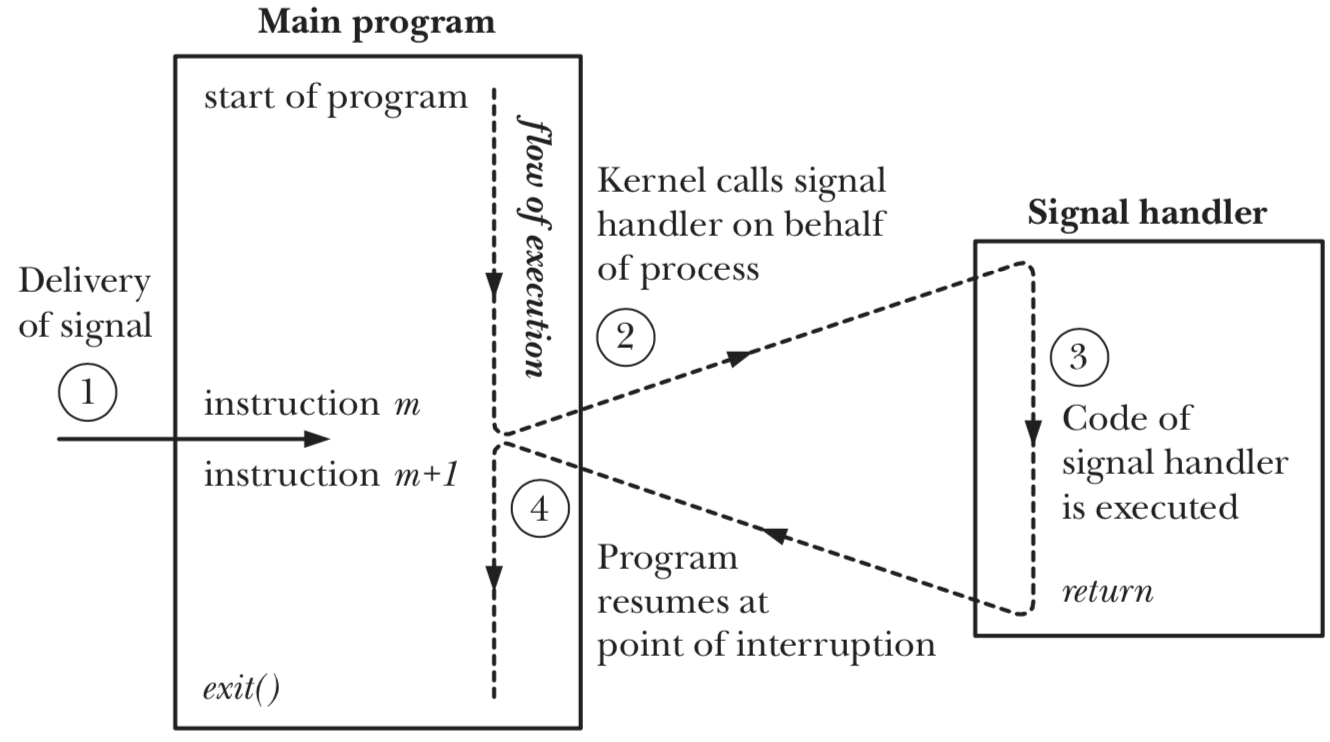
\includegraphics[width=0.8\textwidth]{images/sighandler.png}
	\end{center}


\end{frame}


\begin{frame}
	\frametitle{Tread Carefully!}

	The content of your signal handler, however, is restricted.

	Because the handler deals with an interrupt and runs between two instructions it is important to make sure that the signal handler doesn't mess anything up.

	If the signal handler runs in the middle of \texttt{malloc} and the signal handler itself calls \texttt{malloc} it could put the memory management in an invalid state!

	We can only use functions that are \alert{reentrant}.


\end{frame}


\begin{frame}
	\frametitle{Do Some Research}

	There are tables of what functions are safe to invoke from within a signal handler.

	In general what you are looking for is a designation of \alert{async-signal safe}.

\end{frame}


\begin{frame}[fragile]
	\frametitle{Blocked}

	To block a signal, unblock one, or just find out what the current state is, the function is:
	\begin{lstlisting}[language=C]
int sigprocmask( int how, const sigset_t * set, sigset_t * old_set );
\end{lstlisting}

	The first argument says what we're trying to do here: \texttt{SIG\_BLOCK}, \texttt{SIG\_UNBLOCK}, \texttt{SIG\_SETMASK}.

	Third argument: updated to the old values (if provided).

\end{frame}


\begin{frame}[fragile]
	\frametitle{I am the Mask you wear...}

	There are some helper functions to fill in the mask:
	\begin{lstlisting}[language=C]
int sigemptyset( sigset_t *set ); /* Initialize an empty sigset_t */
int sigaddset( sigset_t *set, int signal ); /* Add specified signal to set */
int sigfillset( sigset_t *set ); /* Add ALL signals to set */
int sigdelset( sigset_t *set, int signal ); /* Remove specified signal from set */
int sigismember( sigset_t *set, int signal ); /* Returns 1 if true, 0 if false */
\end{lstlisting}

\end{frame}


\begin{frame}[fragile]
	\frametitle{Signal Blocking Example}

	\begin{lstlisting}[language=C]
sigset_t set;
sigset_t previous;

sigemptyset( &set ); /* Initialize set */
sigaddset( &set, SIGINT ); /* Add SIGINT to it */

sigprocmask( SIG_BLOCK, &set, &previous ); /* Add SIGINT to the mask */
/* SIGINT is blocked in this section */
sigprocmask( SIG_SETMASK, &previous, NULL ); /* Restore previous mask */

\end{lstlisting}

\end{frame}


\begin{frame}
	\frametitle{Waiting for a Page}

	If you want to pause your program for a bit until the call is interrupted by a signal, there is the function \texttt{int pause( )}.

	This function always returns -1 and it suspends your program until the signal handler runs.

	This can be useful if we really do need to wait for something...

\end{frame}


\begin{frame}
\frametitle{Pass Your Message.}

\begin{center}
	
\includegraphics[width=0.7\textwidth]{images/pass-message.png}
\end{center}

\end{frame}

\begin{frame}
\frametitle{That... Did Not Help}

To deal with the process ID problem, what we would like is \alert{indirect communication} where the messages are sent to mailboxes (queues).


\begin{center}
	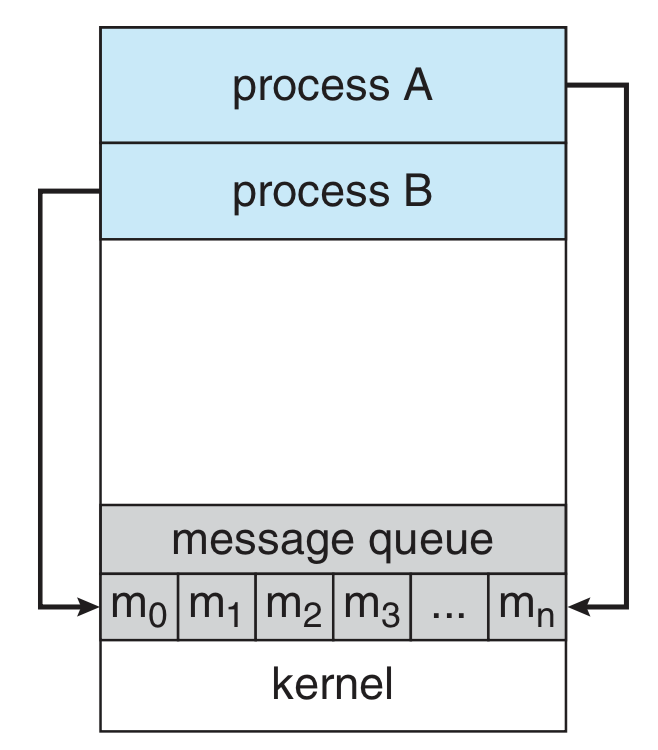
\includegraphics[width=0.4\textwidth]{images/message-passing.png}
\end{center}


\end{frame}


\begin{frame}
\frametitle{UNIX Message Passing}

UNIX gives us this: message queues.

The max sizes and numbers of queues are implementation-specific.

In a real implementation, limits are something you need to consider:
\begin{enumerate}
       \item Wait for the space to be available (block).
       \item Overwrite older messages (sometimes this is what you want).
       \item Discard the current message (leave the old ones as they are).
\end{enumerate}

\end{frame}


\begin{frame}[fragile]
\frametitle{This is Key}

The first step in message-passing is to get a \alert{key} that identifies a specific queue. 

Keys are just integer values, so we would like them to be unique (or close to it).

One method is to generate the key with the ``file to key'' function found in \texttt{sys/ipc.h}:


\begin{lstlisting}[language=C]
key_t ftok( char *pathname, int proj );
\end{lstlisting}

The file does have to exist.

\end{frame}


\begin{frame}
\frametitle{Keep it Secret, Keep it Safe}

Another way we can get a key is using the constant \texttt{IPC\_PRIVATE}. 

If we give the constant in where a \texttt{key\_t} is expected then a guaranteed unique key is returned. 

This method is used when there is a parent and child relationship between the processes that want to communicate.

\end{frame}


\begin{frame}[fragile]
\frametitle{Get the Queue}
Regardless of how we generate the key, we use it to get the queue with the function:
\begin{lstlisting}[language=C]
int msgget( key_t key, int flag );
\end{lstlisting}

\texttt{key}: the key we have generated or \texttt{IPC\_PRIVATE}.

\texttt{flag}: UNIX permissions, optionally \texttt{IPC\_CREAT} with \texttt{IPC\_EXCL}. 

The  permissions follow the UNIX permission standards, e.g. \texttt{0600}.

\texttt{IPC\_CREAT}: create queue (if does not exist).

\texttt{IPC\_EXCL}: fail if trying to create and queue already exists.

Returns: the queue ID.

\end{frame}


\begin{frame}[fragile]
\frametitle{What does a message look like?}

Unlike in a lot of other contexts, here, the message has a defined structure: 

\begin{lstlisting}[language=C]
struct msgbuf {
    long mtype;
    char mtext[1];
};
\end{lstlisting}

\begin{center}
	
\includegraphics[width=0.4\textwidth]{images/zoolander.jpg}
\end{center}

\end{frame}

\begin{frame}[fragile]
\frametitle{Not Quite...}


\begin{center}
	
\includegraphics[width=0.4\textwidth]{images/yesbutno.jpg}
\end{center}


Whatever message type you want to send has to have the first part be a long value; anything is fine after that.

\begin{lstlisting}[language=C]
struct pirate_msgbuf {
    long mtype;  /* must be positive */
    struct pirate_info {
        char name[30];
        char ship_type;
        int notoriety;
        int cruelty;
        int booty_value;
    } info;
};
\end{lstlisting}

\end{frame}

\begin{frame}[fragile]
\frametitle{Sending Data}
\begin{lstlisting}[language=C]
int msgsnd( int msqid, const void *ptr, size_t nbytes, int flag );
\end{lstlisting}

\texttt{msgid}: queue ID.

\texttt{ptr}: message to send.

\texttt{nbytes}: size of the message.

\texttt{flag}: 0 for blocking, \texttt{IPC\_NOWAIT} for return with error if queue full.

\end{frame}


\begin{frame}[fragile]
\frametitle{Receiving Data}
\begin{lstlisting}[language=C]
ssize_t msgrcv( int msqid, void *ptr, size_t nbytes, long type, int flag );
\end{lstlisting}

\texttt{msgid}: queue ID.

\texttt{ptr}: where the message will go.

\texttt{nbytes}: size of the message.

\texttt{type}: kind of message you want.

\texttt{flag}: 0 for blocking, \texttt{IPC\_NOWAIT} for return with error if queue empty.

\end{frame}

\begin{frame}[fragile]
\frametitle{Type Options}
\begin{itemize}
	\item \texttt{type == 0}
	\item \texttt{type > 0}
	\item \texttt{type < 0}
\end{itemize}
\end{frame}

\begin{frame}[fragile]
\frametitle{Destroy!}
\begin{lstlisting}[language=C]
int msgctl( int msqid, int command, struct msqid_ds * buf );
\end{lstlisting}

\texttt{msgid}: queue ID.

\texttt{command}:  \texttt{IPC\_RMID} to delete the queue.

\texttt{buf}: use NULL.

This immediately deletes the queue and all messages inside!

\end{frame}


\begin{frame}[fragile]
\frametitle{Example of Message Passing}

\begin{lstlisting}[language=C]
struct msg {
  long mtype;
  int data;
};

int main( int argc, char** argv ) { 
    int msgqid = msgget( IPC_PRIVATE, 0666 | IPC_CREAT );

    int pid = fork();
    if ( pid > 0 ) { /* Parent */
        struct msg m;
        m.mtype = 42; 
        m.data = 252;
        msgsnd( msgqid, &m, sizeof( struct msg ), 0 );
    } else if ( pid == 0 ) { /* Child */
       struct msg m2; 
       msgrcv( msgqid, &m2, sizeof( struct msg ), 42, 0 );
       printf("Received %d!\n", m2.data );
       msgctl( msgqid, IPC_RMID, NULL );
    }   
    return 0;
}
\end{lstlisting}


\end{frame}





\end{document}

